% 02-metodologija.tex — Methodology (TASK §F.3).
\section{Metodologija}
\label{sec:metodologija}

Metodologija slijedi tok obradnog lanca koji obuhvaća prijem i provjeru mrežnih podataka,
izračun zglobnih kanala, kauzalno filtriranje, preslikavanje na zglobove robota
i komunikaciju s robotom. Opisuju se načela i one odluke koje se vide u
rezultatima.

\subsection{Prijem podataka i analiza frekvencije}

Izvor emitira poze krutih tijela kao UDP datagrame sa sekvencijskim brojem i
vremenskom oznakom, na izvornoj frekvenciji od 120 Hz. Prijemnik iz
sekvencijskog broja detektira gubitak i nepravilan redoslijed, a iz vremena
dolazaka procjenjuje stvarnu frekvenciju i njezinu stabilnost. Upravljačka
petlja ne troši okvire redom nego uvijek uzima najnoviji, a zaostatak u
međuspremniku odbacuje jer je pri radu u stvarnom vremenu stara informacija
štetnija od preskočene. Kad novi okvir ne stigne, zadržava se posljednja valjana
vrijednost umjesto interpolacije, čime se u upravljački signal ne unosi dodatno
kašnjenje. Živi izvor temelji se na protokolu NatNet, a identifikatori krutih
tijela dohvaćaju se službenim SDK klijentom, koji čita definiciju modela iz
inačice NatNet 4.0; sve nizvodno identično je putu s reproduciranom snimkom.

\subsection{Zglobni kanali iz poza krutih tijela}

Svaki segment --- nadlaktica, podlaktica i šaka --- nosi pet reflektirajućih
markera, a u sustavu Motive taj je skup markera definiran kao kruto tijelo
(slika~\ref{fig:markeri}). Zahtjev zadatka od najmanje tri markera po segmentu
time je premašen, i to namjerno. Konfiguracija s tri markera po segmentu
isprobana je prva; premda je geometrijski dovoljna, nema redundancije, pa je već i
djelomično zaklanjanje jednog markera rušilo rekonstrukciju krutog tijela i
prekidalo emitiranje poze. Dva dodatna markera po segmentu daju redundanciju uz
koju sustav Motive nastavlja rješavati pozu i kad dio markera ispadne iz vidnog
polja. Rezultat nije samo robusnija snimka nego i puna poza segmenta, to jest pozicija i
kvaternion orijentacije.

\begin{figure}[htbp]
  \centering
  \IfFileExists{figures/markers_digital_twin.png}{%
    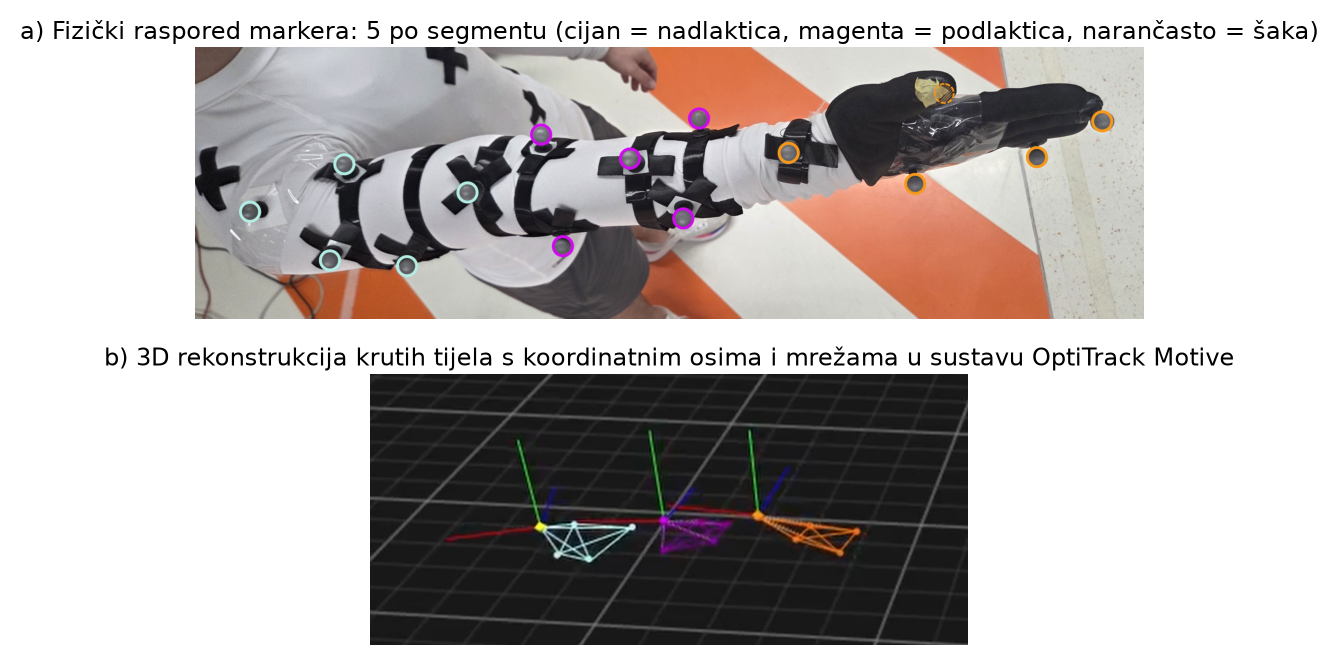
\includegraphics[width=\columnwidth]{figures/markers_digital_twin.png}}{%
    \IfFileExists{figures/markers_detail_crop.jpg}{%
      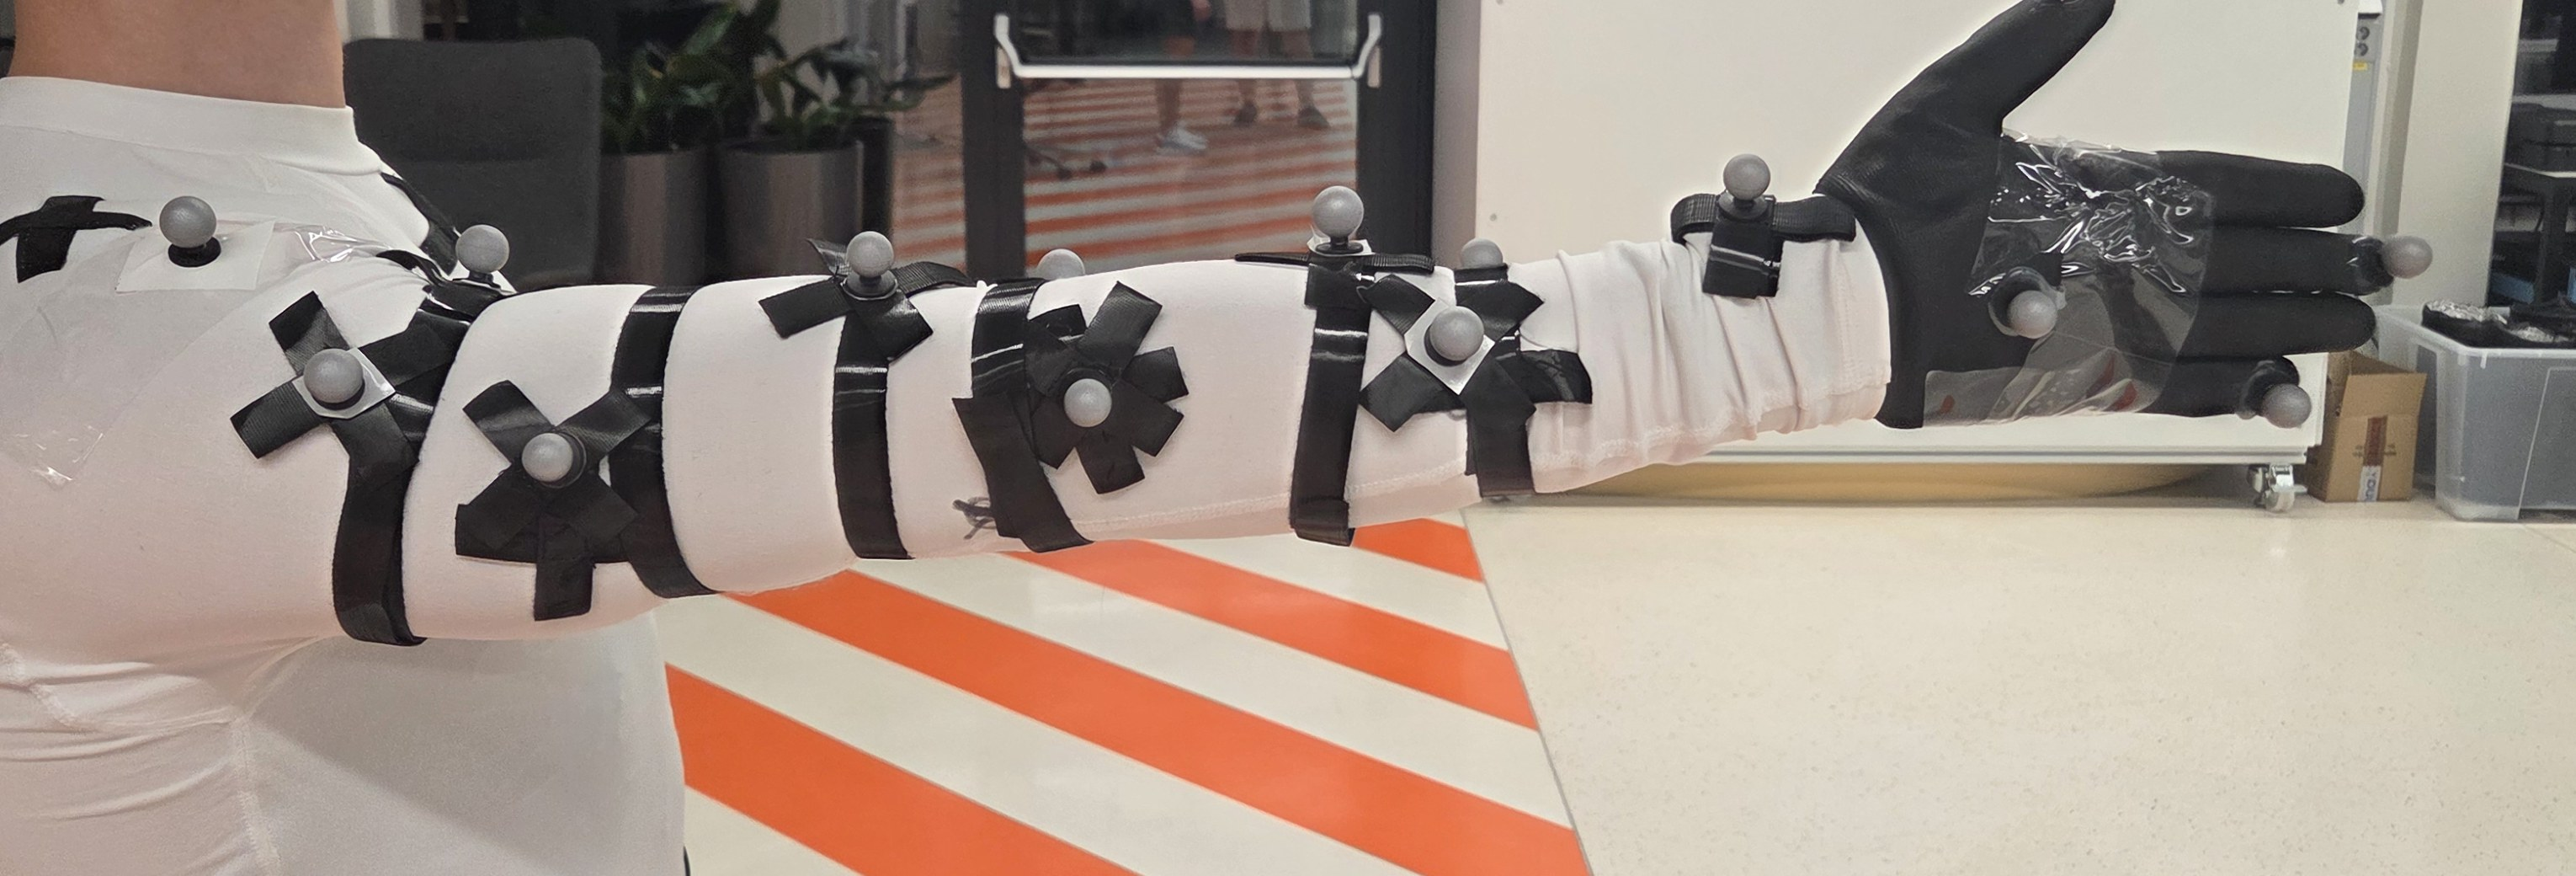
\includegraphics[width=\columnwidth]{figures/markers_detail_crop.jpg}}{%
      \fbox{\parbox[c][2.4cm][c]{0.9\columnwidth}{\centering Detalj markera}}}}
  \caption{Postav markera i digitalni model s prikazom a) fizičkog rasporeda od pet markera po segmentu na ruci operatera te b) rekonstrukcije triju krutih tijela s lokalnim koordinatnim sustavima u programskom paketu Motive.}
  \label{fig:markeri}
\end{figure}

\textbf{Kut lakta} računa se pozicijski, iz triju ishodišta krutih tijela $\mathbf{p}_\text{rame}$, $\mathbf{p}_\text{lakat}$ i $\mathbf{p}_\text{zapešće}$. Iz njih se tvore vektori segmenata
\begin{equation}
  \vec{u} = \mathbf{p}_\text{lakat} - \mathbf{p}_\text{rame}, \quad \vec{v} = \mathbf{p}_\text{zapešće} - \mathbf{p}_\text{lakat},
  \label{eq:vektori}
\end{equation}
a kut fleksije lakta dobiva se numerički stabilnim izrazom
\begin{equation}
  \theta = \operatorname{atan2}\!\big(\lVert \vec{u}\times\vec{v}\rVert,\;
  \vec{u}\cdot\vec{v}\big),
  \label{eq:atan2}
\end{equation}
koji je dobro uvjetovan u cijelom rasponu, za razliku od izravnog $\arccos$
skalarnog umnoška. Kut je definiran kao odstupanje od ispružene ruke i
\emph{neovisan je o mjerilu}, pa duljine segmenata pojedinog korisnika ne treba
kalibrirati.

\textbf{Preostalih pet kanala} izvodi se iz relativnih orijentacija. Za svaki
par segmenata računa se relativna rotacija u odnosu na referentnu pozu snimljenu
pri pokretanju, a iz nje se Eulerovom dekompozicijom izdvaja tražena komponenta.
Pri tome zakret i nagib nadlaktice u odnosu na referentni sustav daju dva kanala ramena,
a rotacija šake u odnosu na podlakticu daje fleksiju i devijaciju zapešća.
Aksijalna komponenta uzeta je iz rotacije podlaktice, a ne šake, jer je mjerena
rotacija oko uzdužne osi šake premalena i spregnuta s ostalim osima. Eulerove
sekvence, indeksi i predznaci nisu pretpostavljeni nego određeni kalibracijom iz
šest izoliranih pokreta, jer ovise o tome kako su lokalne osi krutih tijela
definirane u sustavu Motive; kalibracija je za rame odabrala sekvencu ZXY, a za
zapešće XYZ.

\textbf{Singularnosti.} Orijentacijski put izbjegava gimbal-problem tako što se
rotacije kroz cijeli lanac vode kvaternionima, a u Eulerove kutove prelaze tek
na kraju, u sekvenci odabranoj tako da radni raspon ostane daleko od
degeneracije. Pozicijski kut lakta iz izraza~(\ref{eq:atan2}) numerički je stabilan
u cijelom radnom rasponu, uključujući gotovo ispruženu ruku, gdje bi zapis preko
arkus kosinusa imao beskonačnu derivaciju i milimetarski šum markera pretvarao u
stupnjeve. Pri kolinearnosti nije definirana os rotacije $(\mathbf{u} \times
\mathbf{v})/\lVert \mathbf{u} \times \mathbf{v} \rVert$, no sam kut ostaje
određen. Kut degenerira tek kad ishodišta krutih tijela padnu jedno na drugo,
pa se prag postavlja na duljine $\lVert \mathbf{u} \rVert$ i $\lVert \mathbf{v}
\rVert$; ispod njega se zadržava posljednja valjana vrijednost.

\textbf{Osjetljivost.} Utjecaj mjernog šuma na izračunati kut ispitan je Monte
Carlo perturbacijom pozicija markera; rezultat je u
poglavlju~\ref{sec:rezultati}.

\subsection{Kauzalno filtriranje}

Sirovi kut sadrži visokofrekvencijski šum i fiziološki tremor koje treba
potisnuti bez velikog kašnjenja. Klasično niskopropusno filtriranje unosi fazno
kašnjenje nepovoljno za rad u stvarnom vremenu \cite[str.~2]{zhu2022}, a
nekauzalni postupci poput Savitzky--Golayjeva traže buduće uzorke i primjenjivi
su samo izvanmrežno. Primarni je filtar zato \emph{One-Euro} \cite{casiez2012},
eksponencijalni zaglađivač prvog reda s dinamičkom prilagodbom,
\begin{equation}
  \hat{x}_k = \alpha_k x_k + (1 - \alpha_k)\hat{x}_{k-1}, \quad \alpha_k = \frac{1}{1 + \frac{1}{2\pi f_c T_e}},
  \label{eq:one_euro}
\end{equation}
pri čemu se granična frekvencija $f_c$ linearno prilagođava procijenjenoj brzini promjene prema izrazu
\begin{equation}
  f_c = f_{c,\min} + \beta \, |\hat{\dot{x}}_k|,
  \label{eq:one_euro_fc}
\end{equation}
gdje je $\hat{\dot{x}}_k$ filtrirana diskretna derivacija signala uz fiksnu graničnu frekvenciju $d_c = 1{,}0$\,Hz, $T_e$ period takta, $f_{c,\min}=1{,}0$\,Hz minimalna granična frekvencija i $\beta=0{,}007$ koeficijent brzinske osjetljivosti. Pri mirnoj ruci dominira niska frekvencija koja uklanja podrhtavanje, dok se pri brzom zamahu granična frekvencija automatski podiže i smanjuje kašnjenje.

Kao referenca uspoređeni su kauzalni Butterworthov filtar drugog reda s graničnom frekvencijom 6\,Hz i eksponencijalni pomični prosjek s $\alpha=0{,}2$. Svaki zglob ima vlastitu instancu filtra.

Jedna posljedica te izvedbe pokazala se bitnom i vraća se u
poglavlju~\ref{sec:rezultati}. Filtri su konstruirani za frekvenciju upravljačke
petlje, a ažuriraju se samo kad stigne nova vrijednost kanala. Ako se ulaz
osvježava rjeđe od takta, stvarna granična frekvencija filtra pada razmjerno tom
odnosu i filtar zaglađuje jače nego što je projektiran.

\subsection{Preslikavanje na zglobove robota}

Zglobove robota označavamo 1-baziranom oznakom J1--J6 (J1 baza, J2 rame,
\textbf{J3 lakat}, J4--J6 tri zgloba zapešća), u skladu s nazivljem upravljačke
jedinice. Svaki kanal ide na jedan zglob afinom transformacijom
\begin{equation}
  q_j = q_{j,\mathrm{home}} + s_j\,k_j\,(\theta_j - \theta_{j,\mathrm{home}}),
  \label{eq:mapiranje}
\end{equation}
gdje je $q_{j,\mathrm{home}}$ referentni položaj zgloba, $\theta_{j,\mathrm{home}}$
vrijednost kanala u referentnoj pozi ruke, $k_j$ pojačanje i
$s_j\in\{-1,+1\}$ predznak smjera. Pojačanja nisu jedinična jer nagib ramena ima
$k=2{,}2$, lakat $k=1{,}5$, zapešća $k=1{,}2$, a zakret ramena $k=1{,}0$, čime
se ograničeni raspon ljudskog pokreta u referentnoj pozi razvlači preko
upotrebljivog raspona robota. Predznak je invertiran na nagibu ramena i fleksiji
zapešća da bi se smjerovi poklopili. Ta dva podatka nisu kozmetička --- bez njih
se ulazni i izlazni kut ne mogu uspoređivati, na što se vraćamo pri definiciji
mjere vjernosti.

Obvezni dio zadatka, preslikavanje jednog anatomski podudarnog zgloba, ostvaren
je kao kanal lakta na J3 unutar iste jednadžbe~(\ref{eq:mapiranje}). Savijanje
ljudskog lakta savija lakat robota, pa preslikavanje ostaje intuitivno, a
podudarnost zglobova znači da inverzna kinematika nije potrebna nigdje u lancu.

\subsection{Sigurnosni sloj}

Naredba prije slanja prolazi kroz četiri uzastopna sloja, a to su ograničenje brzine
promjene zgloba, ograničenje raspona oko referentne poze, zadržavanje posljednje
naredbe kad je signal stariji od praga i zaustavljanje izlaza. Prva dva sloja
djeluju stalno i normalan su dio rada, pa zaustavljanje na njima ne bi imalo
smisla; zaustavljanje se okida gumbom za zaustavljanje u nuždi, istekom signala
ili programskim pozivom. Svaki sloj po taktu upisuje zastavicu u zapis, pa je
naknadno moguće pokazati koliko je često i u kojem trenutku djelovao, umjesto
tvrditi da postoji.

\subsection{Komunikacija i mjerenje}

Naredbe se šalju sučeljem RTDE, koje omogućuje sinkroniziranu razmjenu podataka u stvarnom vremenu bez narušavanja vremenskih svojstava upravljačke jedinice; opis sučelja i njegove programske ovojnice daju Lindvig i suradnici \cite{lindvig2025}, čiji metapodaci nisu provjereni s izvornim dokumentom. Programska arhitektura implementira model proizvođač--potrošač s dva neovisna \textit{threada} (prijamnim \textit{threadom} za mrežne podatke i radnim \textit{threadom} upravljačke petlje), u skladu s nalazom da \textit{multi-thread} asinkrona obrada bitno smanjuje kašnjenje u robotskoj teleoperaciji \cite[str.~2]{zainudin2025}. Upravljačka petlja radi na frekvenciji od 125 Hz. Taj je takt odabran jer se nalazi tik iznad izvorišnih 120 Hz sustava OptiTrack, čime se izbjegava nepotrebno trošenje računalnih resursa, dok sučelje RTDE na robotu UR3e podržava frekvencije do 500 Hz.

Tijekom rada kontinuirano se bilježe dva toka podataka. Prvi tok mjeri vremenske karakteristike tako što za svaki pojedini takt bilježi razliku između trenutka primitka okvira na mrežno sučelje i trenutka slanja RTDE naredbe robotu. Ta veličina obuhvaća izračun kinematičkih kutova, filtriranje, provjeru sigurnosnih slojeva i pripremu mrežnog paketa, a u radu se dosljedno naziva latencijom obrade. Drugi tok mjeri kutove, pri čemu se po svakom taktu i zglobu bilježe sirovi ulazni kut, filtrirana vrijednost, ciljna vrijednost, poslana naredba te stvarni kut robota očitan izravno iz internih enkodera preko RTDE telemetrije. Usporedba stvarnog kuta robota s ulaznim kutom ruke omogućuje precizno razlučivanje pojedinačnih doprinosa kašnjenju i pogrešci praćenja.

\textbf{Ispitivanje gubitka paketa.} Otpornost upravljačkog lanca na gubitak UDP paketa ispitana je pri pet nominalnih stopa, od 0 do 30\,\%, determinističkim modeliranjem gubitka nad zajedničkom baznom putanjom snimljenom na robotu. Sustav prati ponašanje pri ispadu pojedinih datagrama tako što pri gubitku okvira zadržava posljednju primljenu valjanu pozu bez interpolacije, čime se sprječava unošenje faznog kašnjenja. Istodobno se mjeri prirast starosti signala i provjerava stabilnost zglobova robota kako bi se potvrdilo da sustav ostaje potpuno stabilan i operativan znatno ispod sigurnosnog praga zaustavljanja.

\FloatBarrier
